\section{Pruebas}
Para comprobar el funcionamiento de los programas se usaron los siguientes archivos wav.\\
Para realizar el filtrado mediante el producto en frecuencia, se uso como entrada para el programa de la FFT el siguiente archivo:
\begin{figure}[H]
	\centering
	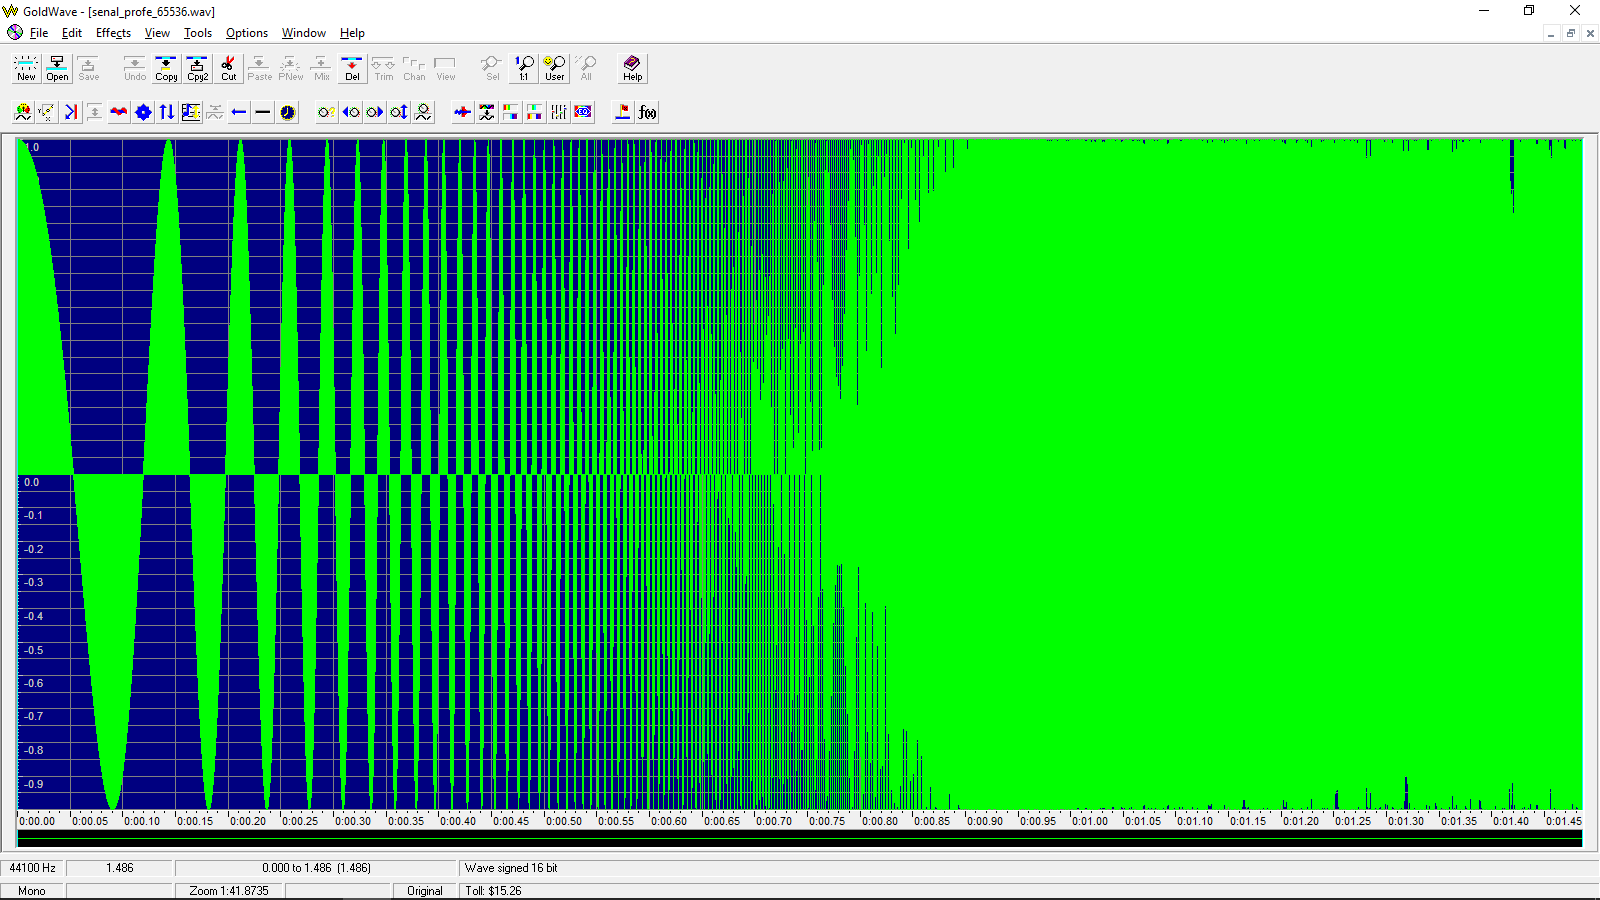
\includegraphics[scale=.35]{img/entrada.png}
	\caption{Archivo de entrada para la FFT}
	\label{fig:prueba1}		
\end{figure}
El cual tiene una frecuencia de muestreo de 44100 muestras/s y una duración de 1.486 segundos.\\ Esa duración fue seleccionada debido a que combinado con la frecuencia de muestreo, el número de muestras obtenidas es cercana a una potencia de dos, la cantidad de muestras que recibe la FFT debe ser una potencia de dos para que funcione correctamente.\\La función usada en el archivo fue: cos(2*pi*t*(exp(log(20)+n/N*6.6))).\newpage
La salida obtenida del programa FFT fue la siguiente:
\begin{figure}[H]
	\centering
	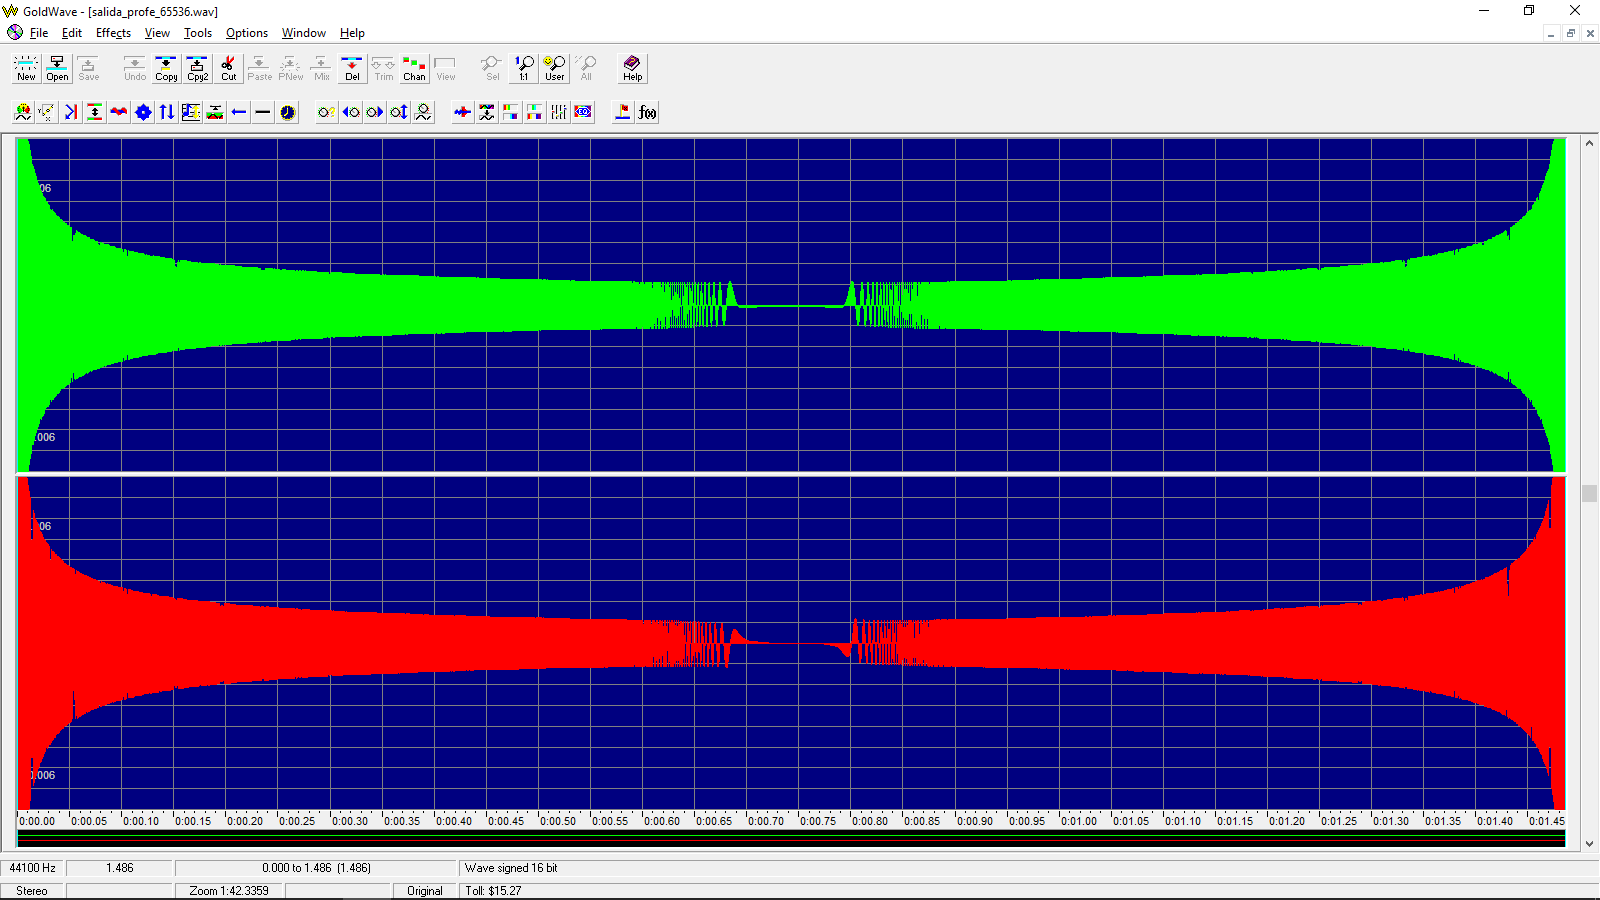
\includegraphics[scale=.35]{img/salidaTDF.png}
	\caption{Salida FFT}
	\label{fig:prueba2}		
\end{figure}
El filtro para realizar el producto se muestra en la siguiente Figura, el filtro fue creado como un archivo wav de 2 canales para simular que el filtro se encuentra en el dominio de la frecuencia, además de que el filtro fue diseñado para ser un filtro ideal (el filtro tiene la misma frecuencia de muestreo y duración que la señal de entrada, y se uso la siguiente función para crearlo: f(x)=(step(n)-step(n-1486))+step(n-(65536-1486))).
\begin{figure}[H]
	\centering
	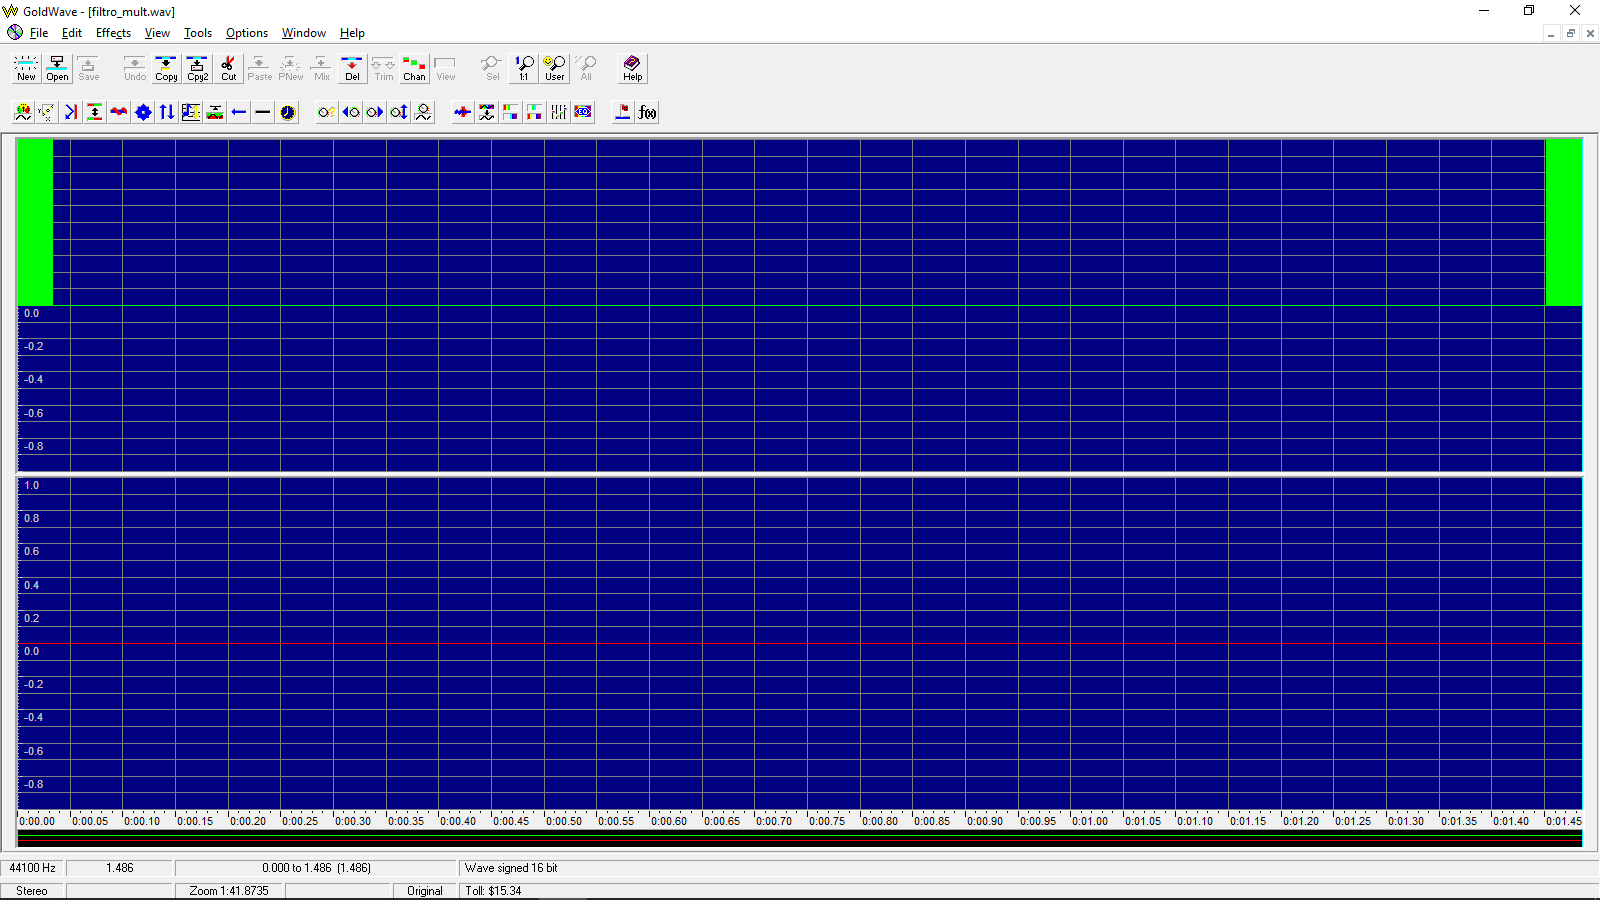
\includegraphics[scale=.3]{img/filtro.png}
	\caption{Filtro ideal en frecuencia}
	\label{fig:prueba2sd}		
\end{figure}
Ambos archivos (salida de FFT y el filtro) se multiplicaron y se obtuvo la siguiente la salida:
\begin{figure}[H]
	\centering
	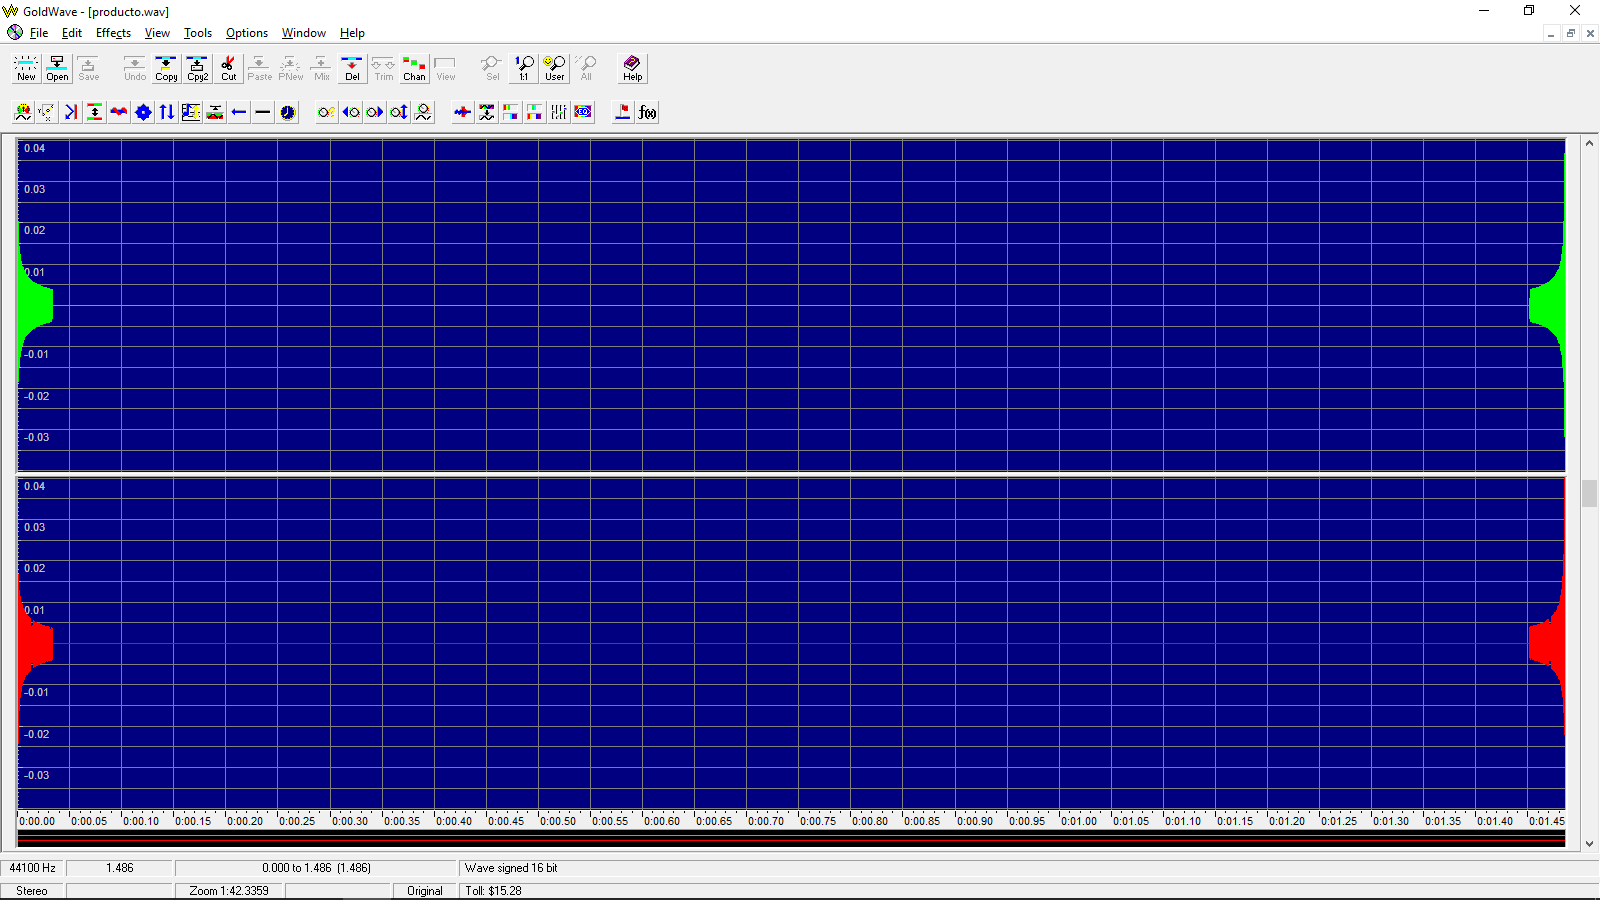
\includegraphics[scale=.35]{img/producto.png}
	\caption{Salida del programa de multiplicación}
	\label{fig:prueba2s}		
\end{figure}
Finalmente, la salida obtenida de la multiplicación fue ingresado al programa que calcula la FFT Inversa, para regresar del dominio de frecuencia al del tiempo.
\begin{figure}[H]
	\centering
	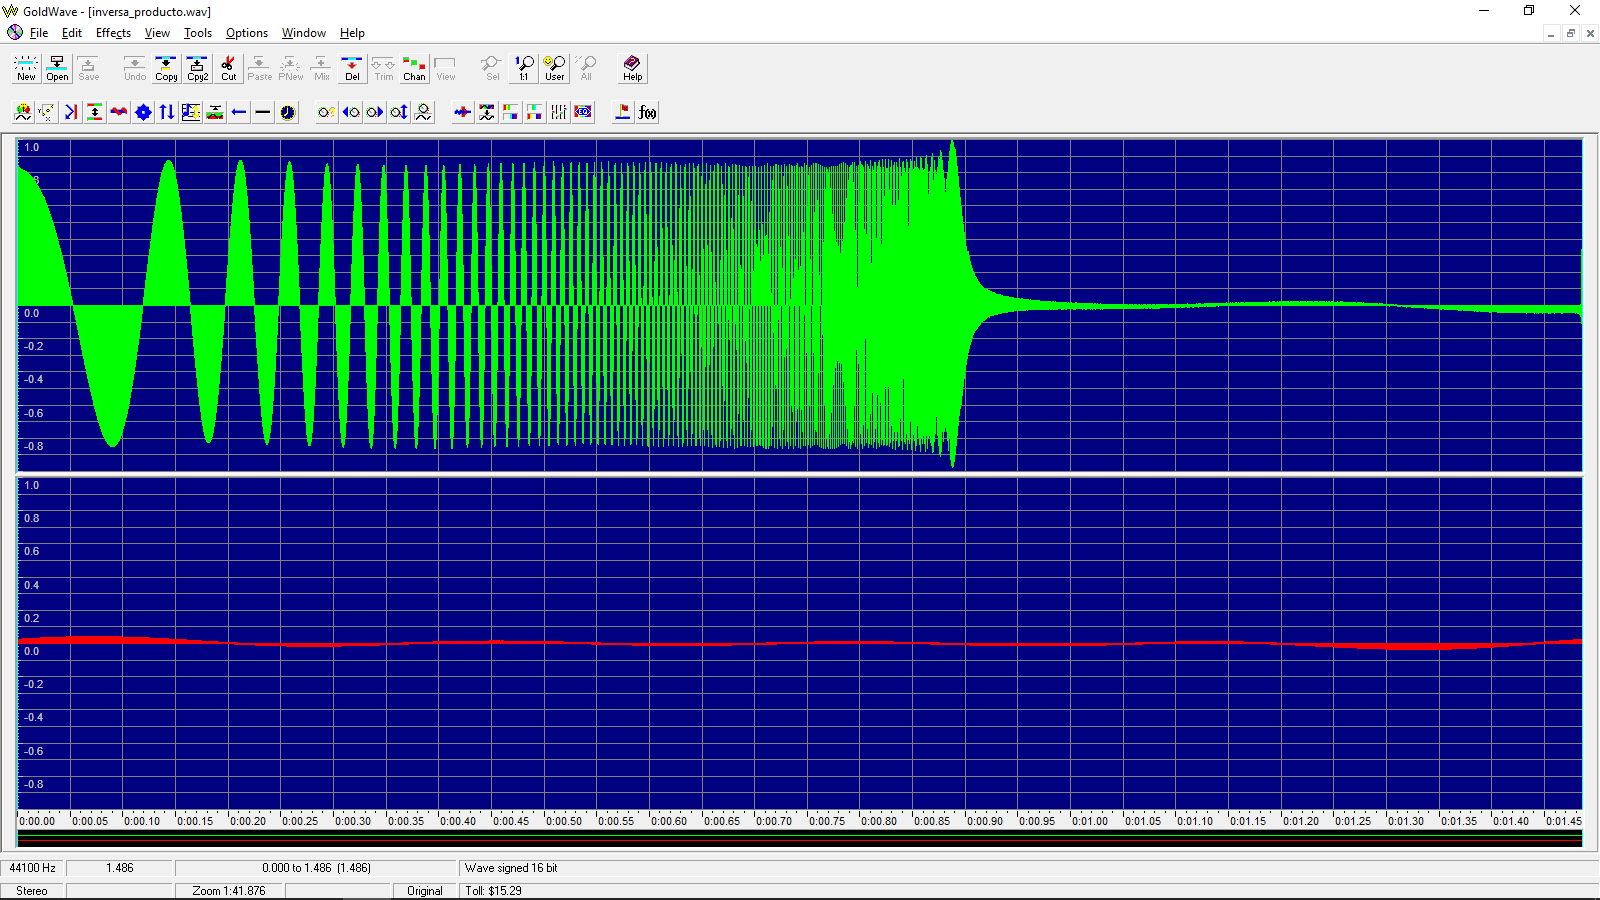
\includegraphics[scale=.35]{img/salida.png}
	\caption{Salida obtenida FFT Inversa}
	\label{fig:preba2s}		
\end{figure}
Para comprobar si el funcionamiento de los programas fue el correcto, se realizó el filtrado de la señal original mediante el uso de Goldwave:
\begin{figure}[H]
	\centering
	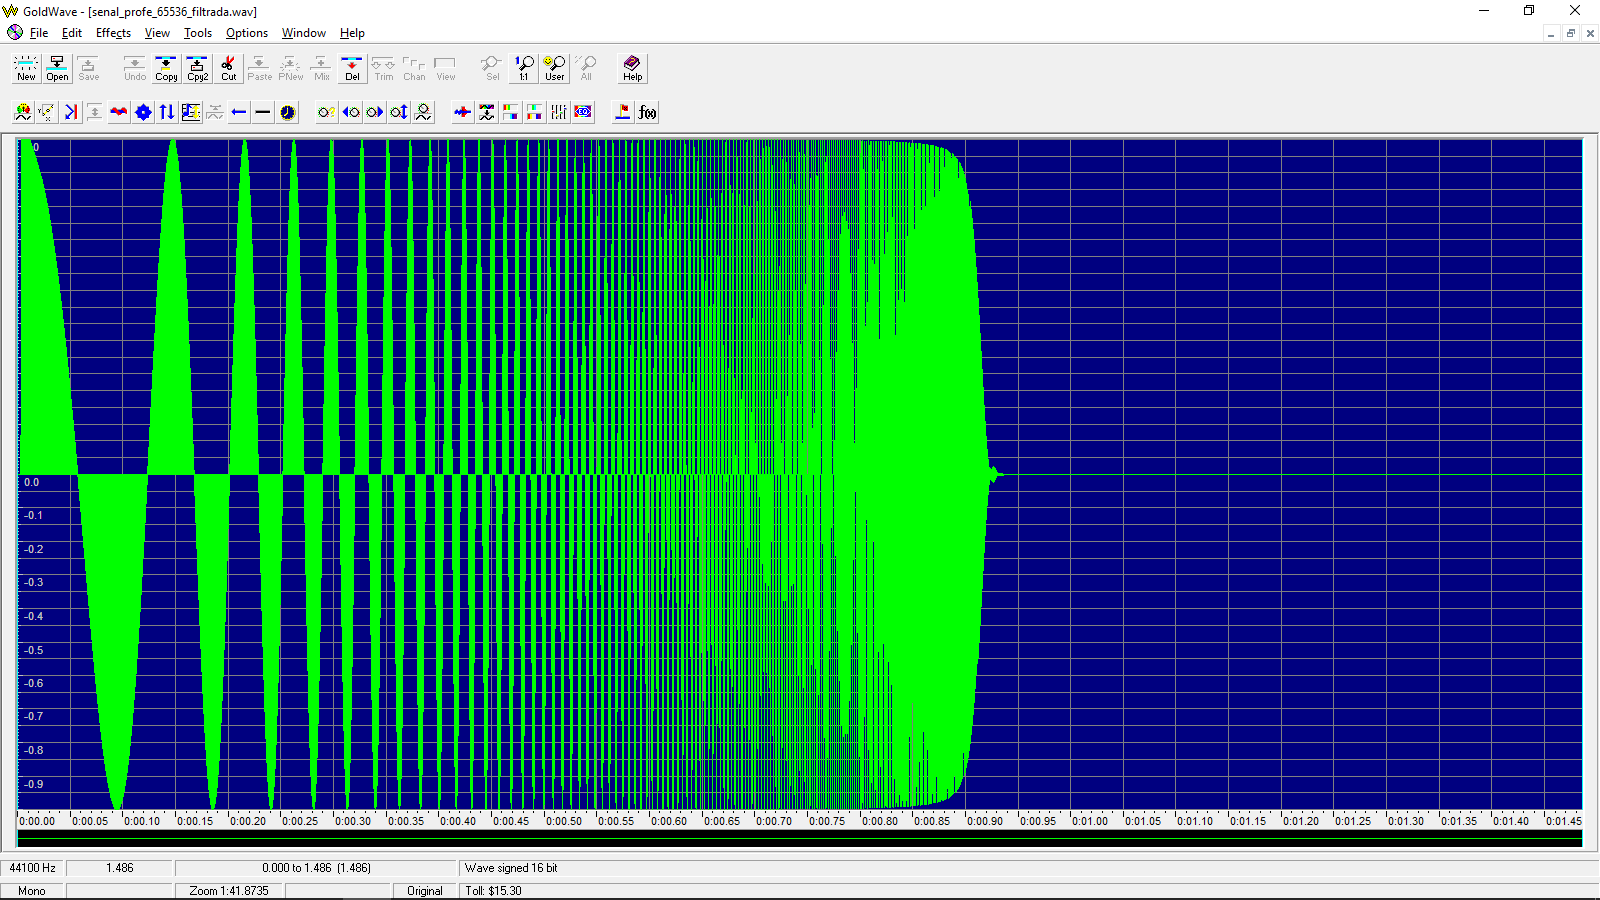
\includegraphics[scale=.35]{img/salida_goldwave.png}
	\caption{Filtrado de la señal original mediante Goldwave}
	\label{fig:preba2}		
\end{figure}
Como se puede observar, el filtrado se realizo correctamente y es muy similar al realizado por Goldwave.\\ Como fue mencionado anteriormente, la FFT tiene un mejor rendimiento (menor tiempo de ejecución) que la TDF, a continuación se muestra un gráfico, del tiempo promedio (en segundos) que tarda la TDF en procesar N muestras.
\begin{figure}[H]
	\centering
	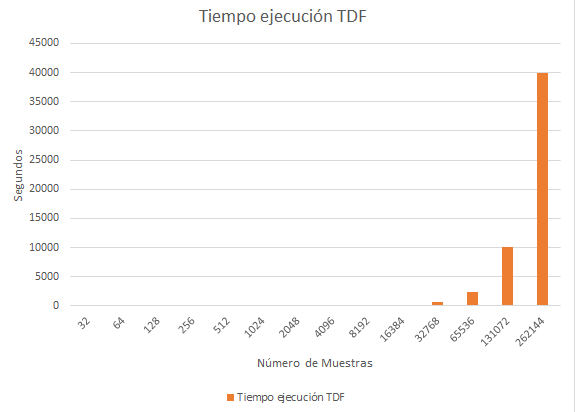
\includegraphics[scale=1]{img/tiempo_tdf.png}
	\caption{Tiempos de ejecución de la TDF}
	\label{fig:prebSDa2}		
\end{figure}
Ahora, se muestra otro gráfico de tiempos de ejecución pero usando la FFT, en la que se puede notar una enorme diferencia:
\begin{figure}[H]
	\centering
	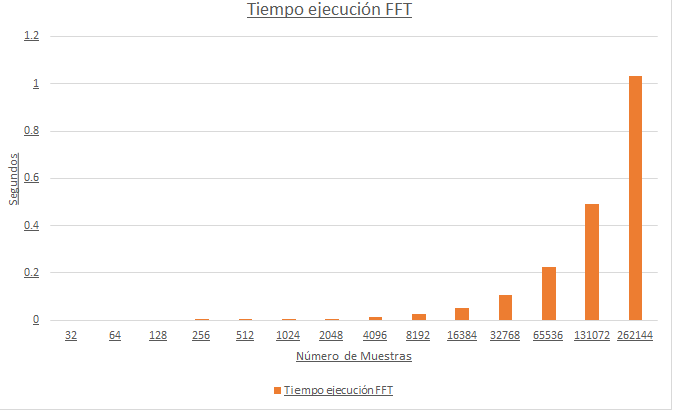
\includegraphics[scale=.88]{img/tiempo_fft.png}
	\caption{Tiempos de ejecución de la FFT}
	\label{fig:prebsdSDa2}		
\end{figure}
Mientras que la TDF puede tardarse cerca de 12 horas en completarse si recibe 262,144 muestras, la FFT se tarda cerca de 1.1 segundos en completarlo. Por lo cual, se puede observar la eficiencia del segundo algoritmo en comparación con el primero.\\
El último gráfico, muestra una comparación entre ambas:
\begin{figure}[H]
	\centering
	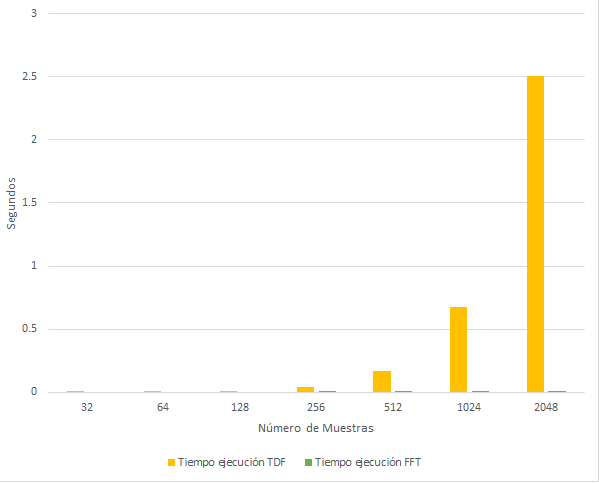
\includegraphics[scale=.88]{img/comparacion.png}
	\caption{Comparación entre la TDF y la FFT}
	\label{fig:prebsdDa2}		
\end{figure}